\section{Polarisation - S.276f, S.278}

\subsection{Begriff}
\begin{itemize}
\item Polarisation ist festgelegt durch die Schwingungsebene der elektrischen Feldstärke des Lichtes.
\item Natürliches Licht ist unpolarisiert, d.h. es enthält Licht aller Polarisationsrichtungen, also in allen Schwingungsebenen.
\end{itemize}

\subsection{Polarisationsfilter}
\begin{itemize}
\item In eine einzige Richtung polarisiertes Licht wird zu 100\% durchgelassen, wenn sicher der Filter in Transmissionsrichtung befindet. Bei 90\degree zur Trasmissionsrichtung wird es zu 100\% abgeschirmt.
\item Malus'sches Gesetz: Intensität $I_1$ vor Filter; $I_2$ nach Filter
\item $I_2 = I_1 \cdot cos^2(\Theta)$
\end{itemize}

\subsection{Brewster-Winkel}
\begin{itemize}
\item Licht kann auch durch Reflexion polarisiert werden. Wenn das Licht im Brewter-Winkel auftrifft, wird der reflektierte Strahl vollständig polarisiert.
(E-Feld steht dann parallel zur Reflexionsebene)
\item Bedingung für vollständige Polarisation: Winkel zwischen reflektiertem und gebrochenem Strahl muss gleich 90\degree sein.
\item $\beta = 90\degree - \alpha_B$
\item $\frac{\sin{\alpha_B}}{\sin{90\degree - \alpha}} = \frac{n_2}{n_1}$ \tabto{4cm}; siehe Brechungsgesetz
\item $\frac{\sin{\alpha_B}}{\cos{\alpha_B}} = \tan{\alpha_B} = n_2$ \tabto{4cm}; $n_1$ ist 1 für Luft bzw. Vakuum

\begin{figure}[h!]
\centering 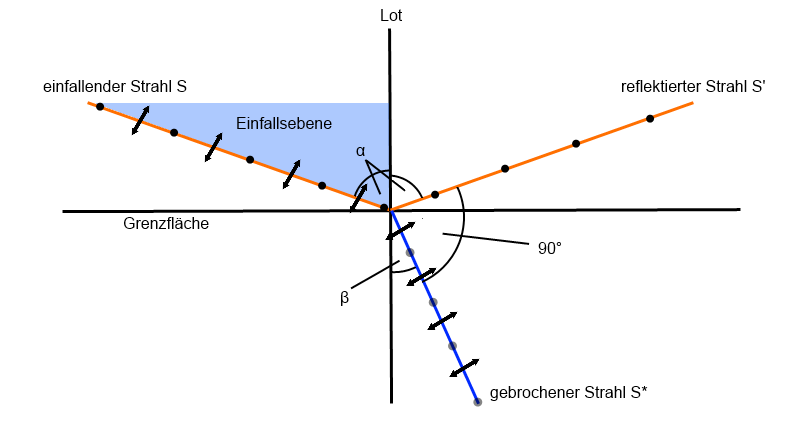
\includegraphics[width=0.8\textwidth]{brewster_winkel}
\caption{Abbildung von \url{http://phy.wdfiles.com/local--files/polarisiertes-licht-c-j/Brewster\%20Winkel\%204.png}}
\end{figure}

\end{itemize}




\section{Hallwachs-Experiment und seine Folgen}
\begin{itemize}
\item Die geladene Zinkplatte eines Ladungsmesser wird mit weißem Licht bestrahlt: Keine Veränderung des Ausschlags der Nadel. Keine Veränderung bei hinzunehmen weiterer, identischer Lichtquellen.
\item Wiederholung des Versuches mit Ultraviolettlicht, welches ein kürzere Wellenlänge besitzt: Ausschlag der Nadel wird kleiner.
\begin{itemize}
	\item Elektronen wurden aus der Metallplatte gelöst
	\item Energie der Welle abhängig von der Wellenlänge und \textbf{nicht} von der Intensität:\\ Widerspruch zur klassischen Wellentheorie
\end{itemize}
\end{itemize}

\section{Fotoeffekt - Experiment 8.11 S.282}
\begin{itemize}
\item Eine Fotozelle wird mit UV-Licht bestrahlt, dadurch werden Elektronen $e^-$ aus der Kathode ausgelöst (Natrium). Es wird eine Gegenspannung $U_{max}$ angelegt und so lange erhöht, bis kein Strom I mehr gemessen wird.

Die herausgeschlagenen $e^-$ besitzen eine kinetische Energie $E_{kin}$. Durch die Gegenspannung müssen sie gegen ein elektrisches Feld "ankämpfen". Wenn kein Strom I mehr gemessen wird ist die elektrische Energie $E_{el} = U \cdot e$ gleich der kinetischen Energie $E_{kin} = \dfrac{1}{2} m v^2$.
\item Im nächsten Schritt wird die maximale kinetische Energie (uns interessieren nur die schnellsten Elektronen) der Photonenenergie abzüglich der minimalen Austrittsarbeit, die notwendig ist um ein Elektron überhaupt aus der Platt zu lösen, gleich gesetzt.

$E_{kin,max} = E_{phot} - W_A$ ; Der Unterschied zwischen Arbeit und Energie ist philosophischer Natur, d.h. Energie und Arbeit haben die selben Einheiten.
\item Daraus folgt die Einstein'sche Gleichung: \\ 
$E_{kin,max} = h \cdot f - W_A$ \tabto{0.5\textwidth} ; $E_{phot} = h \cdot f$ \\
$E_{el} = E_{kin,max}$ \\
$e \cdot U = h \cdot f - W_A$ \tabto{0.5\textwidth} ; $E_{el} = e \cdot U$
\item Das Plack'sches Wirkungsquantum $h$ ist konstant: $h = 6,626\cdot10^{-34} Js$ [$\frac{kg \ m^2}{s^2} \cdot s$]
\item Die Grenzfrequenz $f_{gr}$ ist die Frequenz ab der Elektronen ausgelöst werden, sie ist Material abhängig.

$W_A = h \cdot f_{gr} \rightarrow f_{gr} = \frac{W_A}{h}$
\end{itemize}

\begin{figure}[h!]
\centering 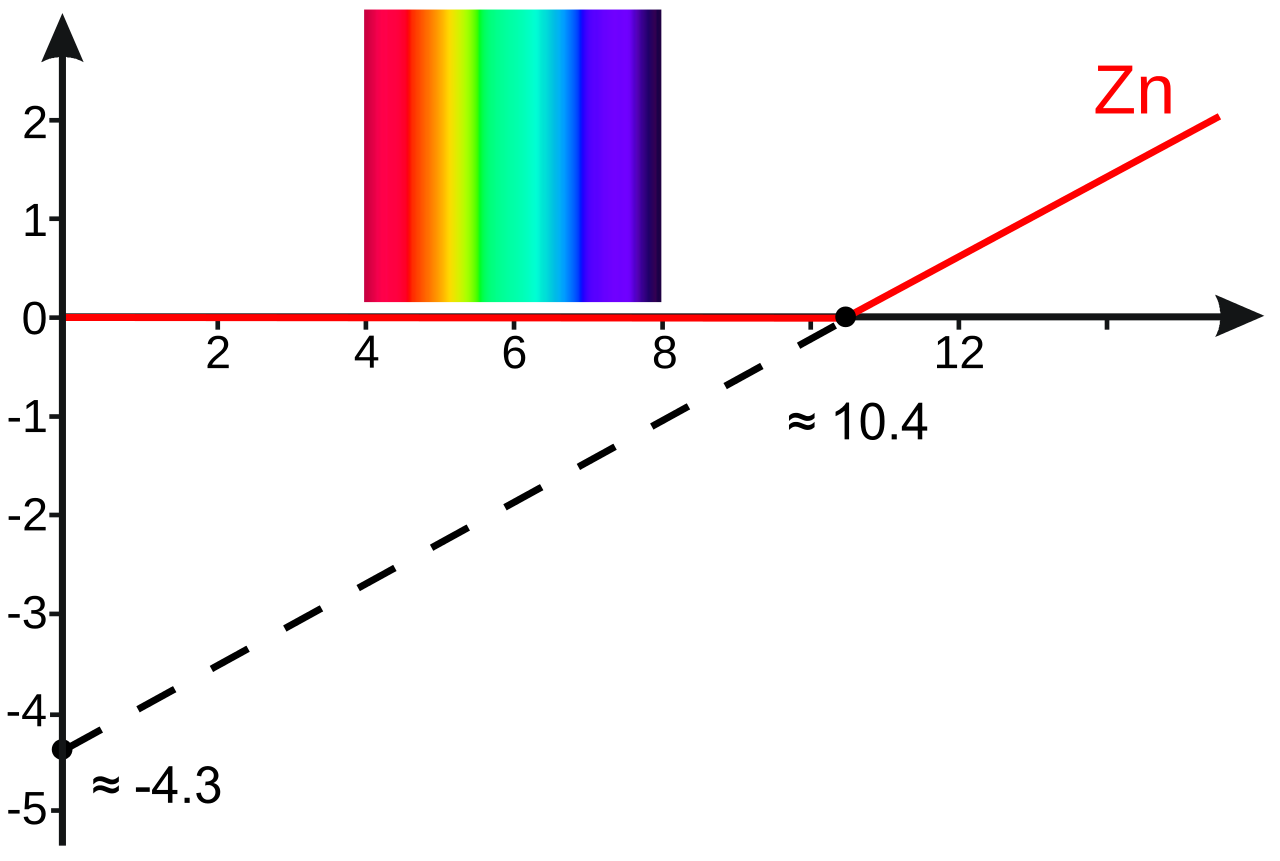
\includegraphics[width=0.8\textwidth]{Photoelectric_effect_diagram_no_label}
\caption{Abbildung von: \url{https://upload.wikimedia.org/wikipedia/commons/thumb/5/54/Photoelectric\_effect\_diagram\_no\_label.svg/1280px-Photoelectric\_effect\_diagram\_no\_label.svg.png}}
\end{figure}

\section{Licht als Teichen und als Welle}
\begin{itemize}
\item Licht als Welle:
	\begin{itemize}
	\item Bei Wellenoptik, Hygens'sches Prinzip, elektromagnetische Welle (E-Feld, B-Feld)
	\item Brechung, Reflexion, Polarisation
	\item Doppelspalt, Einzelspalt
	\end{itemize}
\item Licht als Teilchen:
	\begin{itemize}
	\item Immer wenn von Licht als Photon die Rede ist.
	\item Fotoeffekt, Compton-Streuung
	\item Photonenimpuls
	\end{itemize}
\end{itemize}

\section{Photonenimpuls}
\begin{itemize}
\item Der Impuls $\vec{p}$ eines beliebigen Körpers mit Masse ist definiert als: 

$\vec{p} = m \cdot \vec{v}$
\item Photonen haben aber keine Ruhemasse. Ihre Masse lässt sich nur durch Umformen der Gleichung der speziellen Relativitätstheorie $E = mc^2$ ermitteln.

$m = \frac{E}{c^2}$

daraus folgt:

$\vec{p} = \frac{E}{c^2} \cdot \vec{c}$ \tabto{0.5\textwidth} ; $\vec{v} = \vec{c}$ da Photonen sich stets mit Lichtgeschwindigkeit fortbewegen.

$\vec{p} = \frac{h \cdot f}{\vec{c}}$ \tabto{0.5\textwidth} ; $E_{phot} = h \cdot f$

$\vec{p} = \frac{h}{\lambda \cdot f}$ \tabto{0.5\textwidth} ; $c = \lambda \cdot f$

$\vec{p} = \frac{h}{\lambda}$
\item Das heißt das, dass alles mit einem Impuls eine Wellenlänge hat, \referenz{subsec:DeBroglie}
\item Nice to know: $F = \frac{\Delta p}{\Delta t}$
\end{itemize}

\subsection{Elastischer Stoß}
\begin{itemize}
\item Bei einem elastischen Stoß bleibt die Summe der kinetischen Energien der Stoßpartner unverändert.

$\frac{1}{2}m_1 \cdot v_1^2 = \frac{1}{2}m_1 \cdot (v'_1)^2 + \frac{1}{2}m_2 \cdot (v'_2)^2$
\item Wenn $m_1 << m_2$ (wie bei Experiment Lichtmühle bzw. Photon Reflektor) ist $v'_1 \approx -v_1$ und $\vec{p'} \approx -2 \vec{p}$
\end{itemize}

\subsection{Unelastischer Stoß}
\begin{itemize}
\item Der Vorgang ist nicht reibungsfrei, es geht kinetische Energie "verloren" (Umwandlung in Wärme).
\item Beispiel Elektronen auf schwarze Fläche, es kommt nur zum einfachen Impulsübertrag, die verlorene Energie wird in Wärme umgewandelt.
\end{itemize}


\subsection{De Broglie} \label{subsec:DeBroglie}
\begin{itemize}
\item Jedes Teilchen mit Impuls hat eine Wellenlänge. Die De Broglie-Wellenlänge $\lambda_{dB}$ berechnet sich folgendermaßen: $\lambda_{dB} = \frac{h}{p}$
\end{itemize}

\section{Elektronenbeugung...}
\begin{itemize}
\item Aufgrund der De Broglie-Wellenlänge haben Elektronen eine Wellenlänge, wenn sie einen Impuls besitzen.
\item Die Wellenlänge eines Elektron ist bei bestimmten Konfigurationen groß genug, dass Interferenzerscheinungen auftreten (Das Elektron \textbf{verhält} sich wie eine Welle, ist aber keine.)
\item Theoretisch lässt sich seinen Wellenlänge $\lambda$ durch das Gleichsetzen der Gleichung des Impulses $\vec{p}=m\cdot\vec{v}$ mit der Formel für den Photonenimpuls $\vec{p}=\frac{h}{\lambda}$:

$m\cdot\vec{v}=\frac{h}{\lambda}$ \tabto{0.5\textwidth} ; umstellen nach $\lambda$

$\lambda = \frac{h}{m \cdot v} $

\item Um die Geschwindigkeit $v$, bei einem Versuch mit Elektronenbeschleunigung durch ein elektrisches Feld, zu ersetzen, setzt man zunächst die Gleichungen der kinetischen Energie $E_{kin}$ mit der Gleichung der Elektrischen $E_{el}$ gleich und formt anschließend nach $v$ um.

$\frac{1}{2} m_e \cdot v^2 = e \cdot U_a$ \tabto{0.5\textwidth} ; $U_a$ ist die Beschleunigungsspannung, mit der das Elektron in dem jeweiligen Versuch beschleunigt wurde.

$v = \sqrt{\frac{2e \cdot U_a}{m_e}}$

durch Einsetzen folgt dann:

\Large $\lambda = \frac{h \sqrt{m_e}}{m \cdot \sqrt{2e \cdot U_a}} $
\end{itemize}

\subsection{...an Grafit}
\begin{itemize}
\item Da Elektronen demnach eine sehr kleine Wellenlänge haben, benutzt man oft Kristalle um Interferenzmuster zu erzeugen.
\item An den Netzebenen des Kristalls, in denen die Atome regelmäßig angeordnet sind, werden Elektronen, ähnlich wie Licht an dünnen Schichten (Glimmer), gestreut.
\item Auf dem Leuchtschirm der Röhre kommt es je nach Gangunterschied über die verschiedenen Netzebenen zu Maxima und Minima.
\item Wichtig: Bei Grafit haben die Atome in einer Ebene einen anderen Abstand d zu einander, als die Atome zwischen den Ebenen. Es gibt als zwei "Spaltabstände" und folglich auch zwei Maxima 1. (2.,...,n.) Ordnung.

\item Der Gangunterschied $\delta = 2d\cdot\sin{\alpha} $ für konstruktive Interferenz muss ein natürliches vielfaches der Wellenlänge $\lambda$ sein.

$n \cdot \lambda = 2d \cdot \sin{\alpha}$

\Large $\sin{\alpha} = \frac{n \cdot \lambda}{2d}$ Bragg'sche Bedingung / Gleichung
\end{itemize}

Achtung in der Zeichnung ist $\alpha$ mit $\Theta$ vertauscht!

\begin{figure}[h!]
\centering 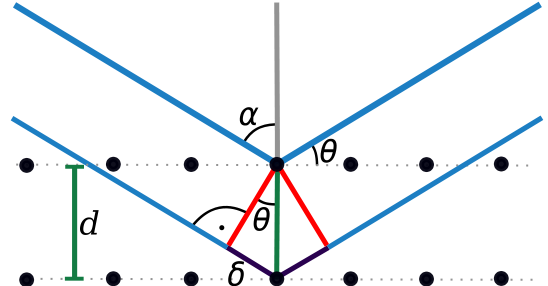
\includegraphics[width=0.8\textwidth]{Streuung_an_Graphit}
\caption{Abbildung von: \url{https://upload.wikimedia.org/wikipedia/commons/thumb/c/ca/Bragg.svg/548px-Bragg.svg.png}}
\end{figure}



\subsubsection{Versuch}
\begin{itemize}
\item Im Versuch wird ein Elektronenstrahl auf einen Graphitkristall geleitet, an diesem kommt es zu Streuung und es bilden sich jeweils zwei ringförmige Maxima auf dem Schirm.
\item Bezeichnet man den Abstand vom Maximum n. Ordnung zum Maximum 0. Ordnung mit $r$ und den Abstand vom Kristall zum Schirm mit $l$ folgt:

$\tan{2\alpha} = \frac{r}{l}$
\item Um die Wellenlänge der Elektronen experimentell zu bestimmen, setzten wir dies Formel mit der Bragg'schen Gleichung gleich.

$2\sin{\alpha} = tan{2\alpha}$

wendet man die Kleinwinkelnäherung an, folgt: \\
\Large $\frac{n\cdot\lambda}{2d}=\frac{r}{l}$

\normalsize

umgestellt nach $\lambda$:\\
\Large $\lambda = \frac{2dr}{n\cdot l}$

\normalsize

ohne Winkelnäherung:\\
\Large $2\cdot\arcsin(\frac{n\cdot \lambda}{2d})=\arctan(\frac{r}{l}) $

\Large $\arcsin(\frac{n\cdot \lambda}{2d})=\frac{1}{2}\cdot\arctan(\frac{r}{l})$ 

\Large $\frac{n\cdot \lambda}{2d}=\sin(\frac{1}{2}\cdot\arctan(\frac{r}{l}))$ 

\Large $\lambda=\sin(\frac{1}{2}\cdot\arctan(\frac{r}{l}))\cdot 2d \cdot \frac{1}{n}$ \tabto{0.5\textwidth} ; meistens ist n=1 

\normalsize

\item Nice to know: Es kommt nur zur Interferenz, wenn die Bragg'sche Gleichung erfüllt ist. Dafür muss $\alpha$, für eine bestimmte Wellenlänge, auch eine bestimmte Größe haben. Im Experiment wird deshalb eine Graphitfolie benutzt, auf der die Kristallgitter in den verschiedensten Anordnungen liegen. So ist statistisch gesehen immer ein Kristall im richtigen Winkel zum Elektronenstrahl.
\end{itemize}

\subsection{...am Doppelstpalt}
\begin{itemize}
\item Grundsätzlich gelten die gleichen Formeln wie bei Interferenz mit Licht. Allerdings muss der Spaltabstand $d$, aufgrund der ebenfalls sehr kleinen Wellenlängen, sehr klein sein, um überhaupt ein Interferenzmuster detektieren zu kommen.\\
Das Interferenz Muster ist so klein, dass man es nur mit einem Elektronenmikroskop sichtbar machen kann.
\item Bedingungen für konstruktive Interferenz: $\delta = n \cdot \lambda$\\
für destruktive Interferenz: $\delta = (n-\frac{1}{2}) \cdot \lambda$
\end{itemize}

\subsubsection{Versuch}
\begin{itemize}
\item Um die Wellenlänge $\lambda$ experimentell herauszufinden, gilt, wenn $d$ der Spaltabstand ist, $a$ der Abstand zum Schirm und $d_k$ der Abstand des k. Maximum zum 0. Maximum ist:

$\tan{\alpha}=\frac{d_k}{a}$ und $\sin{\alpha}=\frac{k \cdot\lambda}{d}$

Dann entweder durch Kleinwinkelnäherung:\\
\Large $\lambda = \frac{d_k \cdot d}{k \cdot a}$

\normalsize oder ohne:

\Large $\lambda = \sin(\arctan(\frac{d_k}{a})) \cdot \frac{d}{k}$
\end{itemize}

\section{Compton-Streuung}
\begin{itemize}
\item Wenn man Photonen mit ausreichend Energie (ab ca. 100keV) auf gebundene Elektronen schießt, wird das Phänomen durch den Photoeffekt beschrieben. Es kommt zur vollständigen Impulsübertragung vom Photon auf das Elektron.
\item Wenn man Photonen gegen ein freies Elektron schießt, wird das Phänomen durch den Compton-Effekt beschrieben:
\begin{itemize}
\item Es kommt nicht immer zu einer vollständigen Impulsübertrag.
\item Wenn nicht der ganze Impuls übertragen wird, kommt es zur Compton-Streuung.
Das Elektron wird in eine Richtung wird durch den Teilimpuls in eine Richtung beschleunigt, und das Photon wird in eine andere abgelenkt.\\
Nach dem Zusammenstoß hat das Photon einen geringeren Impuls, und da seine Geschwindigkeit konstant $c$ ist, ändert sich seine Wellenlänge (sie wird größer).
\begin{comment}\item Durch den Impulserhaltungssatz gilt:\\
Vor Kollision:\\
$p_{gesamt} = p_{Phot} \rightarrow p_{gesamt}=\frac{h}{\lambda}$


Nach Kollision: \\
$p_{gesamt} = p'_{phot} + p_e$

$\frac{h}{\lambda} = \frac{h}{\lambda'} + m_e \cdot v$

$\frac{h}{\lambda} = \frac{h}{\lambda} \cdot \cos{\Theta} + \frac{h}{\lambda} \cdot (1-\cos{\Theta})$ \tabto{0.5\textwidth} ; $c = \lambda * f \rightarrow \lambda = c / f$

$\frac{h}{\lambda} = \frac{h}{\lambda} \cdot \cos{\Theta} + \frac{h}{\lambda} \cdot (1-\cos{\Theta})$





$m_e \cdot v = \frac{h}{\lambda}$ \tabto{0.5\textwidth} ; umstellen nach $\lambda$ 


$\lambda' = \lambda + \Delta\lambda$

$\lambda' - \lambda = \Delta\lambda$

$\lambda' - \lambda = $


$\lambda = \frac{h}{m_e \cdot v}$

\end{comment}

\begin{comment}
Vor Kollision:\\
$p_{gesamt} = p_{phot}$

Nach Kollision: \\
$p_{gesamt} = p'_{phot} + p_{Teilchen, an dem gestreut}$

Für $\Delta p$: \\
$p_{gesamt} - p'_{phot} = \Delta p$ \tabto{0.5\textwidth} ; umstellen nach $p_{gesamt}$ \\
$p_{gesamt} = \Delta p + p'_{phot}$ \\

Einsetzen in die Gesamtgleichung für nach Kollision:\\
$\frac{h}{\Delta \lambda} + \frac{h}{\lambda '} = \frac{h}{\lambda '} + m \cdot v$ \tabto{0.5\textwidth} ; mit $p_{Teilchen, an dem gestreut} = m \cdot v$ \\
$\frac{h}{\Delta \lambda} = m \cdot v$ \\
$\frac{h}{\Delta \lambda \cdot m \cdot v} = 1$ \\
$\Delta \lambda = \lambda_c = \frac{h}{m \cdot v}$ \\


\end{comment}
\end{itemize}
\begin{comment}
\item Compton-Wellenlänge hergeleitet:

Durch den Impulserhaltungssatz gilt:\\

Vor Kollision:\\
$p_{gesamt} = p_{phot}$

Nach Kollision: \\
$p_{gesamt} = p'_{phot} + p_{Teilchen, \ an \ dem \ gestreut}$

Für $\Delta p$: \\
$\Delta p = p_{phot} - p'_{phot}$

$\Delta p = p_{gesamt} - p'_{phot}$ \tabto{0.5\textwidth} ; umstellen nach $p_{gesamt}$

$p_{gesamt} = \Delta p + p'_{phot}$ \\


Einsetzen in die Gesamtgleichung für "nach Kollision": \\
$\frac{h}{\Delta \lambda} + \frac{h}{\lambda '} = \frac{h}{\lambda '} + m \cdot v$ \tabto{0.5\textwidth} ; mit $p_{Teilchen, \ an \ dem \ gestreut} = m \cdot v$

$\frac{h}{\Delta \lambda} = m \cdot v$ \\

Dann noch nach $\Delta \lambda$ umformen und man erhält die Compton Wellenlänge: \\
$\Delta \lambda = \lambda_c = \frac{h}{m \cdot v}$ \\
\end{comment}

Für ein Elektron als Teilchen, an dem gestreut wird, gilt folgende Konstante (Taschenrechner: Konstante 12: "Compton-Wellenlänge des Elektrons"): \\
$\Delta \lambda = \lambda_c = \frac{h}{m_e \cdot v} \approx 2,426 \cdot 10^{-12}m $ \\


\item Wellenlängenänderung in Abhängigkeit des Streuungswinkels $\Theta$:

$\lambda' -\lambda = \frac{h}{m \cdot c}-\frac{h}{m \cdot c} \cos{\Theta}$

$\Delta\lambda = \frac{h}{m \cdot c}(1-\cos{\Theta})$ \tabto{0.5\textwidth} ; $\lambda_c = \frac{h}{m \cdot c}$

$\Delta\lambda = \lambda_c \cdot (1-\cos{\Theta})$

\item Maximum ist bei $\Theta = 180\degree \rightarrow (1-\cos{180\degree})=2$
\item Minimum ist bei $\Theta = 0\degree \rightarrow (1-\cos{0\degree})=0$

\end{itemize}